\documentclass{article}
\usepackage[top=1in, bottom=1in, left=1in, right=1in]{geometry}
% \usepackage{fullpage, fancyhdr}
\usepackage{fullpage}
\usepackage{float}
\usepackage{mathtools}
\usepackage{caption}
\usepackage{subcaption}
\usepackage{portland}
\usepackage{graphicx}
\usepackage{hyperref}
%\usepackage{setspace}
\setlength{\topmargin}{0.0in}
\setlength{\headheight}{0.5in}
\setlength{\headsep}{0in}
\setlength{\footskip}{9pt}


% \pagestyle{fancyplain}
\pagestyle{myheadings}
\voffset=-0.50in
\topmargin=0.00in 
\headsep=0.25in 
\evensidemargin=0in 
\oddsidemargin=0in 
\textwidth=6.6in 
\textheight=10.0in 

\renewcommand{\topfraction}{0.9}	% max fraction of floats at top
\renewcommand{\bottomfraction}{0.8}	% max fraction of floats at bottom
%   Parameters for TEXT pages (not float pages):
\setcounter{topnumber}{2}
\setcounter{bottomnumber}{2}
\setcounter{totalnumber}{4}     % 2 may work better
\setcounter{dbltopnumber}{2}    % for 2-column pages
\renewcommand{\dbltopfraction}{0.9}	% fit big float above 2-col. text
\renewcommand{\textfraction}{0.07}	% allow minimal text w. figs
%   Parameters for FLOAT pages (not text pages):
\renewcommand{\floatpagefraction}{0.7}	% require fuller float pages
% N.B.: floatpagefraction MUST be less than topfraction !!
\renewcommand{\dblfloatpagefraction}{0.7}	% require fuller float pages
% remember to use [htp] or [htpb] for placement
\def\tm{\leavevmode\hbox{$\rm {}^{TM}$}}

\title{Assignment \# 1: Archos 80 XS}
\date{ \today }
\author{Brian Arnberg}

\markright{Brian Arnberg\hfill ELEC 6260 - Embedded Computing Systems\hfill}     
\setlength{\parindent}{0pt}


\begin{document}\label{start}

\begin{titlepage}
	\maketitle
	\thispagestyle{empty}
\end{titlepage}

% Intro
\section*{ Introduction }
This report will discuss the ARCHOS 80 XS. 
The ARCHOS 80 XS is an Android\tm\   based tablet. It is aimed at multimedia applications, and can be integrated into a home entertainment system readily, especially because it is capable of efficiently encoding/decoding 1080p resolution videos.\cite{Main} 

\section*{ Major Components }

% Processors
\subsection*{ Processors }
The CPU, clocked at 1200MHz, is a Rockchip RK3066 with a machine word width of 32 bits.\cite{Second} TheRockchip RK3066 is a dual\--core A9 @ 1.6GHz CPU, which includes a quad\--core mali 400 MP GPU.\cite{rk30xx} Figure~\ref{rk3066} shows the block diagram of the RK3066. The block diagram can be used to quickly assess the functionality of the RK3066.

The Cortex\--A9 is ``designed around the high efficiency, dual\--issue superscalar, out\--of\--order, speculating dynamic length pipeline,'' and implements the ARMv7 architecture.\cite{A9} It offers 2.50 DMIPS/MHz per core and has a Memory Management Unit (MMU) for memory management. The Mali 400, features anti\--aliasing,  API Support for OpenGL ES 1.1/2.0, an AMBA$\textsuperscript{\textregistered}$ AXI bus interface, and a built in MMU.\cite{Mali-400} Both the Cortex\--A9 and the Mali\--400 are well suited to integrate into system\--on\--chip designs, such as the RK3066. 

\begin{figure}[!htbp]
	\centering
	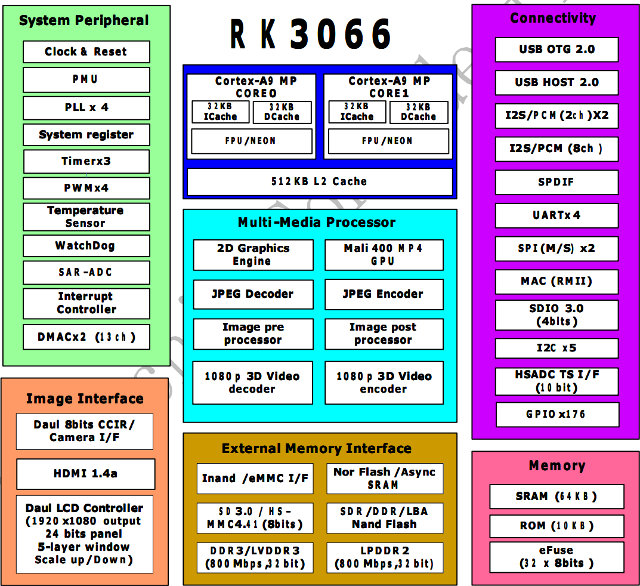
\includegraphics[width=0.95\textwidth]{rk3066.jpg}
	\caption{This is a technical block diagram of the Rockchip RK3066. Both the CPU and the GPU are ARM chips. }
	\label{rk3066}
\end{figure}

\subsection*{ Memory }
The system RAM type is LPDDR2 SDRAM clocked at 400MHz. The system RAM capacity is 1024MiB. The system ROM type is Flash EEPROM.

\subsection*{ Capacity }
The system uses built in flash memory to provide 8GB of storage, but also has a microSD slot which is SDXC compatible up to 64GB.\cite{Main}

\subsection*{ Graphics }
The graphics are processed by the Mali\--400 previously mentioned. The system has a display color depth of 24 bits. It uses an 8'': 1024x768 MVA (Multi\--domain vertical alignment) display, with a pixel density of 160.2 pixels/inch. The video out supports 1920x1080 (or 1080p). The tablet depends on an HDMI Type C connector for video out. 

\subsection*{ Audio }
The tablet supports stereo sounds. The built\--in loudspeakers only support mono sound, while audio out is stereo. The tablet has a 3.5mm plug for audio out, as well as a built\--in microphone for audio in (which is mono sound).

\subsection*{ Touch Screen }
The tablet can be manipulated by the use of a multi-touch screen or by an attachable QWERTY-type keyboard. The touchscreen is capacitive, and is enabled as a 5-point multitouch screen.  

\subsection*{ Interfaces }
The system has a microSD card slot, which is compatible with microSD, microSDHC, Transflash, and microSDXC. It supports High Capacity chips (SD 2.0/HC) up to 32GB, and Extended Capacity chips (SDXC) up to 64GB. The tablet also has a USB 2.0 host/client Hi-Speed (480Mbits/s) port using a USB Series Micro-B (Micro-USB connector. The tablet is capable of using Bluetooth 4.0 (IEEE 802.15) via an internal antenna.  The tablet is also capable of connecting to a Wireless LAN/Wi\--Fi network (either IEEE 802.11b, 802.11g, or 802.11n) via an internal antenna. 

\subsection*{ Satellite Navigation }
The tablet has built\--in GPS support. It uses the GPS Protocol NMEA 0183 and an internal antenna. 

\subsection*{ Digital Camera }
There is a built\--in digital camera. It uses a CMOS type sensor and has a resolution of 1280x1024, or 1.31 MP). When it is acting as a camcorder, it stores the video at 1280x720 pixels and 30 frames/sec. The images will be formatted to JPG, and the videos will be either formatted to 3GP or MPEG4.  

\subsection*{ Power }
The tablet primarily runs off of a battery, but it can be charged via the Micro-USB connector.


%%%%%

% Instruction+Set: 	ARMv7-A
% Built-in_accelerometer: 	Supported

%%%%%

\section*{ System Architecture }
The ARCHOS 80 XS is built on an ARM Cortex-A9 processor, which is based on the ARMv7-A instruction set.

\section*{ Operating System }
The Embedded Operating System is Google Android 4.1.1, Jelly Bean. Jelly Bean is an improved version of Android 4.0. The Home Page for Jelly Bean states that it ``is the fastest and smoothest version of Android yet``. \cite{JellyBean} Jelly Bean is capable of Accessibility features such as ``Gesture Mode,'' focus, ``TalkBack,'' and braille accessibility. It supports instantly sharing photos over Bluetooth using Android Beam. It also supports USB Audio Docks. It has a built\--in web browser, an integrated calendar, built\--in camera support, intelligent data usage management in the background on the SSID, has an improved version of Face Unlock (your face is the system password), internationalization, a built\--in notification system, WiFi networking, News and Weather fetching, voice typing, and many other things. Basically, the Android Operating System allows for all the same basic usability features that are normally associated with a Desktop OS like Windows XP or Linux. In fact, Android is based on an embedded version of the Linux kernel, which allows the ARCHOS 80 XS, and other Android based devices, to take advantage of free and regular software updates.   
% Embedded_Operating;System: 	Google Android 4.1.1
% Operating-System-Kernel: 	Linux

\newpage
\begin{thebibliography}{1}
	\bibitem{Main}
		\url{http://www.archos.com/products/gen10/archos_80xs/index.html?country=us&lang=en}
	\bibitem{Second}
		\url{http://pdadb.net/index.php?m=specs&id=3977&view=1&c=archos_gen10_80_xs}
	\bibitem{rk30xx}
		\url{http://www.cnx-software.com/2012/11/04/rockchip-rk3066-rk30xx-processor-documentation-source-code-and-tools/}
	\bibitem{A9}
		\url{http://arm.com/products/processors/cortex-a/cortex-a9.php?tab=Specifications}
	\bibitem{Mali-400}
		\url{http://www.arm.com/products/multimedia/mali-graphics-hardware/mali-400-mp.php}
	\bibitem{JellyBean}
		\url{http://www.android.com/about/jelly-bean/}
\end{thebibliography}

%  \begin{figure}[htbp]
%   \centering
%   \includegraphics[width=4.0in,keepaspectratio]{E-Field}
%   \caption{\small{ The E-Field pattern produced by the initial code. }}
%   \label{fig:E-Field}
%   \end{figure}
%  \begin{figure}[htbp]
%   \centering
%   \includegraphics[width=4.0in,keepaspectratio]{Power}
%   \caption{\small{ The normalized power pattern of the system.  }}
%   \label{fig:Power}
%   \end{figure}

\label{end}\end{document}


